\section{Zusammenhang Graphentheorie und GraphQL}

GraphQL erlaubt es uns, Typen zu definieren. Ein Type beinhaltet immer mindestens eine Property. Ein Type kann mit einem
Knoten eines Graphens gleichgesetzt werden. Und eine Beziehung zwischen Types als Kante. Hierdurch lässt sich dann
ein Typgraph entwickeln der als Bauplan für reale Graphen dient.
Man nehme zum Beispiel ein Buch und definiere hierfür einen Type

\begin{center}
    \begin{verbatim}
        type Book {
            id: Int
            title: String
        }
    \end{verbatim}
\end{center}

Es exisitiert jetzt ein Objekt Book mit den Eigenschaften id als Integer und title als String.
Repräsentiert als Graphen hätten wir nun einen einfachen Knoten der zwei Datentypen speichert.

\begin{center}
    
\includegraphics[width=\textwidth,height=\textheight,keepaspectratio]{img/book}
\end{center}

Ein Objekt enthält 1 bis n Propertys. Diese Property kann entweder ein Standarddatentyp sein oder auf einen Type verweisen,
dies kann der eigene Type oder auch ein anderer Type sein.
Fügen wir unserem Beispiel des Buches eine Property hinzu mit dem Type Author wobei der Author selbst
wie folgt definiert wird:

\begin{center}
    \begin{verbatim}
        type Book {
            id: Int
            title: String
            author: Author
        }
        type Author {
            id: Int
            name: String
        }
    \end{verbatim}
\end{center}

So fügen wir unserem Graphen einen zusätzlichen Knoten hinzu
Die Beziehung zwischen dem Buch und Author wird durch eine gerichtete Kante zwischen dem Buch und dem Author dargestellt.
Hierdurch ergibt sich folgender Graph:

\begin{center}
    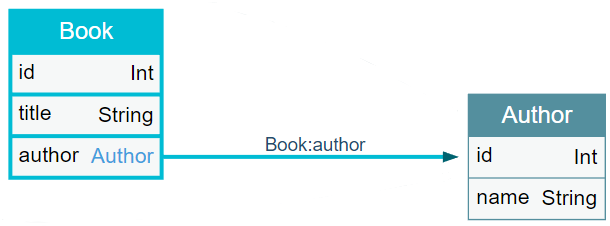
\includegraphics[width=\textwidth,height=\textheight,keepaspectratio]{img/book-author}
\end{center}

Fügen wir dem Author nun auch noch die Property written hinzu, so ergibt sich ein Kreis in diesem Graph.

\begin{verbatim}
    type Book {
        id: Int
        title: String
        author: Author
    }
    type Author {
        id: Int
        name: String
        written: [Books!]
    }
\end{verbatim}

so ergibt sich, dass wir einen zirkulären Graphen haben mit folgender Struktur

\begin{center}
    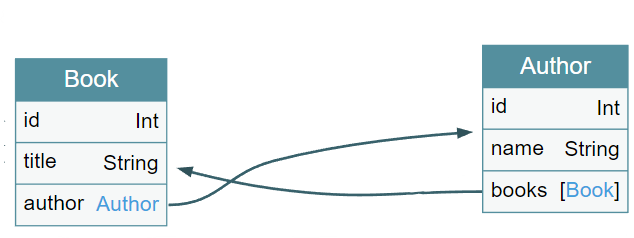
\includegraphics[width=\textwidth,height=\textheight,keepaspectratio]{img/book-author-circle}
\end{center}


Dieses Schema ist ein Bauplan für einen sehr einfachen, zirkulären Graphen der durch GraphQL abgebildet wird.
In Realität können die Graphstrukturen die aus diesem Bauplan resultieren sehr unterschiedlich sein.
Für dieses Beispiel kann das bedeuten, dass folgende beide Graphen korrekt definierte Graphen sind jedoch komplett
andere Möglichkeiten bieten wie man sie abfragen kann. Hierdurch resultiert auch, dass die Abfragen
diverse Möglichkeiten haben je nach den unterliegenden Daten.

\begin{figure}
    \begin{center}
        \begin{tikzpicture}
            \node (1)[abstract, rectangle split, rectangle split parts=2] at (0,0)
                {
                \textbf{Book}
                \nodepart{second} \begin{description}
                                      \item[id:] Integer
                                      \item[title:] String
                \end{description}
            };
            \node (2)[abstract, rectangle split, rectangle split parts=2] at (5,0)
                {
                \textbf{Book}
                \nodepart{second} \begin{description}
                                      \item[id:] Integer
                                      \item[title:] String
                \end{description}
            };
            \node (3)[abstract, rectangle split, rectangle split parts=2] at (10,0)
                {
                \textbf{Book}
                \nodepart{second} \begin{description}
                                      \item[id:] Integer
                                      \item[title:] String
                \end{description}
            };
            \node (4)[abstract, rectangle split, rectangle split parts=2] at (0,5)
                {
                \textbf{Author}
                \nodepart{second} \begin{description}
                                      \item[id:] Integer
                                      \item[name:] String
                \end{description}
            };
            \node (5)[abstract, rectangle split, rectangle split parts=2] at (10,5)
                {
                \textbf{Author}
                \nodepart{second} \begin{description}
                                      \item[id:] Integer
                                      \item[name:] String
                \end{description}
            };
            \draw [->] (4) to node [midway]{ schrieb } (1);
            \draw [->] (4) to node [midway]{ schrieb } (2);
            \draw [->] (5) to node [midway]{ schrieb } (3);

        \end{tikzpicture}
    \caption{3 Bücher, 2 Autoren}
    \end{center}
\end{figure}


\begin{figure}
    \begin{center}
        \begin{tikzpicture}[scale=0.7, transform shape]
            \node (1)[abstract, rectangle split, rectangle split parts=2] at (0,0)
                {
                \textbf{Book}
                \nodepart{second} \begin{description}
                                      \item[id:] Integer
                                      \item[title:] String
                \end{description}
            };
            \node (2)[abstract, rectangle split, rectangle split parts=2] at (4,0)
                {
                \textbf{Book}
                \nodepart{second} \begin{description}
                                      \item[id:] Integer
                                      \item[title:] String
                \end{description}
            };
            \node (3)[abstract, rectangle split, rectangle split parts=2] at (8,0)
                {
                \textbf{Book}
                \nodepart{second} \begin{description}
                                      \item[id:] Integer
                                      \item[title:] String
                \end{description}
            };
            \node (4)[abstract, rectangle split, rectangle split parts=2] at (12,0)
                {
                \textbf{Book}
                \nodepart{second} \begin{description}
                                      \item[id:] Integer
                                      \item[title:] String
                \end{description}
            };
            \node (5)[abstract, rectangle split, rectangle split parts=2] at (16,0)
                {
                \textbf{Book}
                \nodepart{second} \begin{description}
                                      \item[id:] Integer
                                      \item[title:] String
                \end{description}
            };
            \node (6)[abstract, rectangle split, rectangle split parts=2] at (20,0)
                {
                \textbf{Book}
                \nodepart{second} \begin{description}
                                      \item[id:] Integer
                                      \item[title:] String
                \end{description}
            };
            \node (7)[abstract, rectangle split, rectangle split parts=2] at (10,5)
                {
                \textbf{Author}
                \nodepart{second} \begin{description}
                                      \item[id:] Integer
                                      \item[name:] String
                \end{description}
            };
            \draw [->] (7) to node [midway]{ schrieb } (1);
            \draw [->] (7) to node [midway]{ schrieb } (2);
            \draw [->] (7) to node [midway]{ schrieb } (3);
            \draw [->] (7) to node [midway]{ schrieb } (4);
            \draw [->] (7) to node [midway]{ schrieb } (5);
            \draw [->] (7) to node [midway]{ schrieb } (6);
        \end{tikzpicture}
        \caption{6 Bücher, 1 Autor}
    \end{center}
\end{figure}

Definiert man nun, dass es zum Beispiel die StandardQuery "getBookAuthor(id): Author" geben soll. So bedeutet dies,
dass ein Author eines Buches abgefragt werden soll aufgrund der Id eines Buches.

(Hier Graphen einfügen mit Highlight der gewählten Knoten)



